\begin{figure}
    \centering
    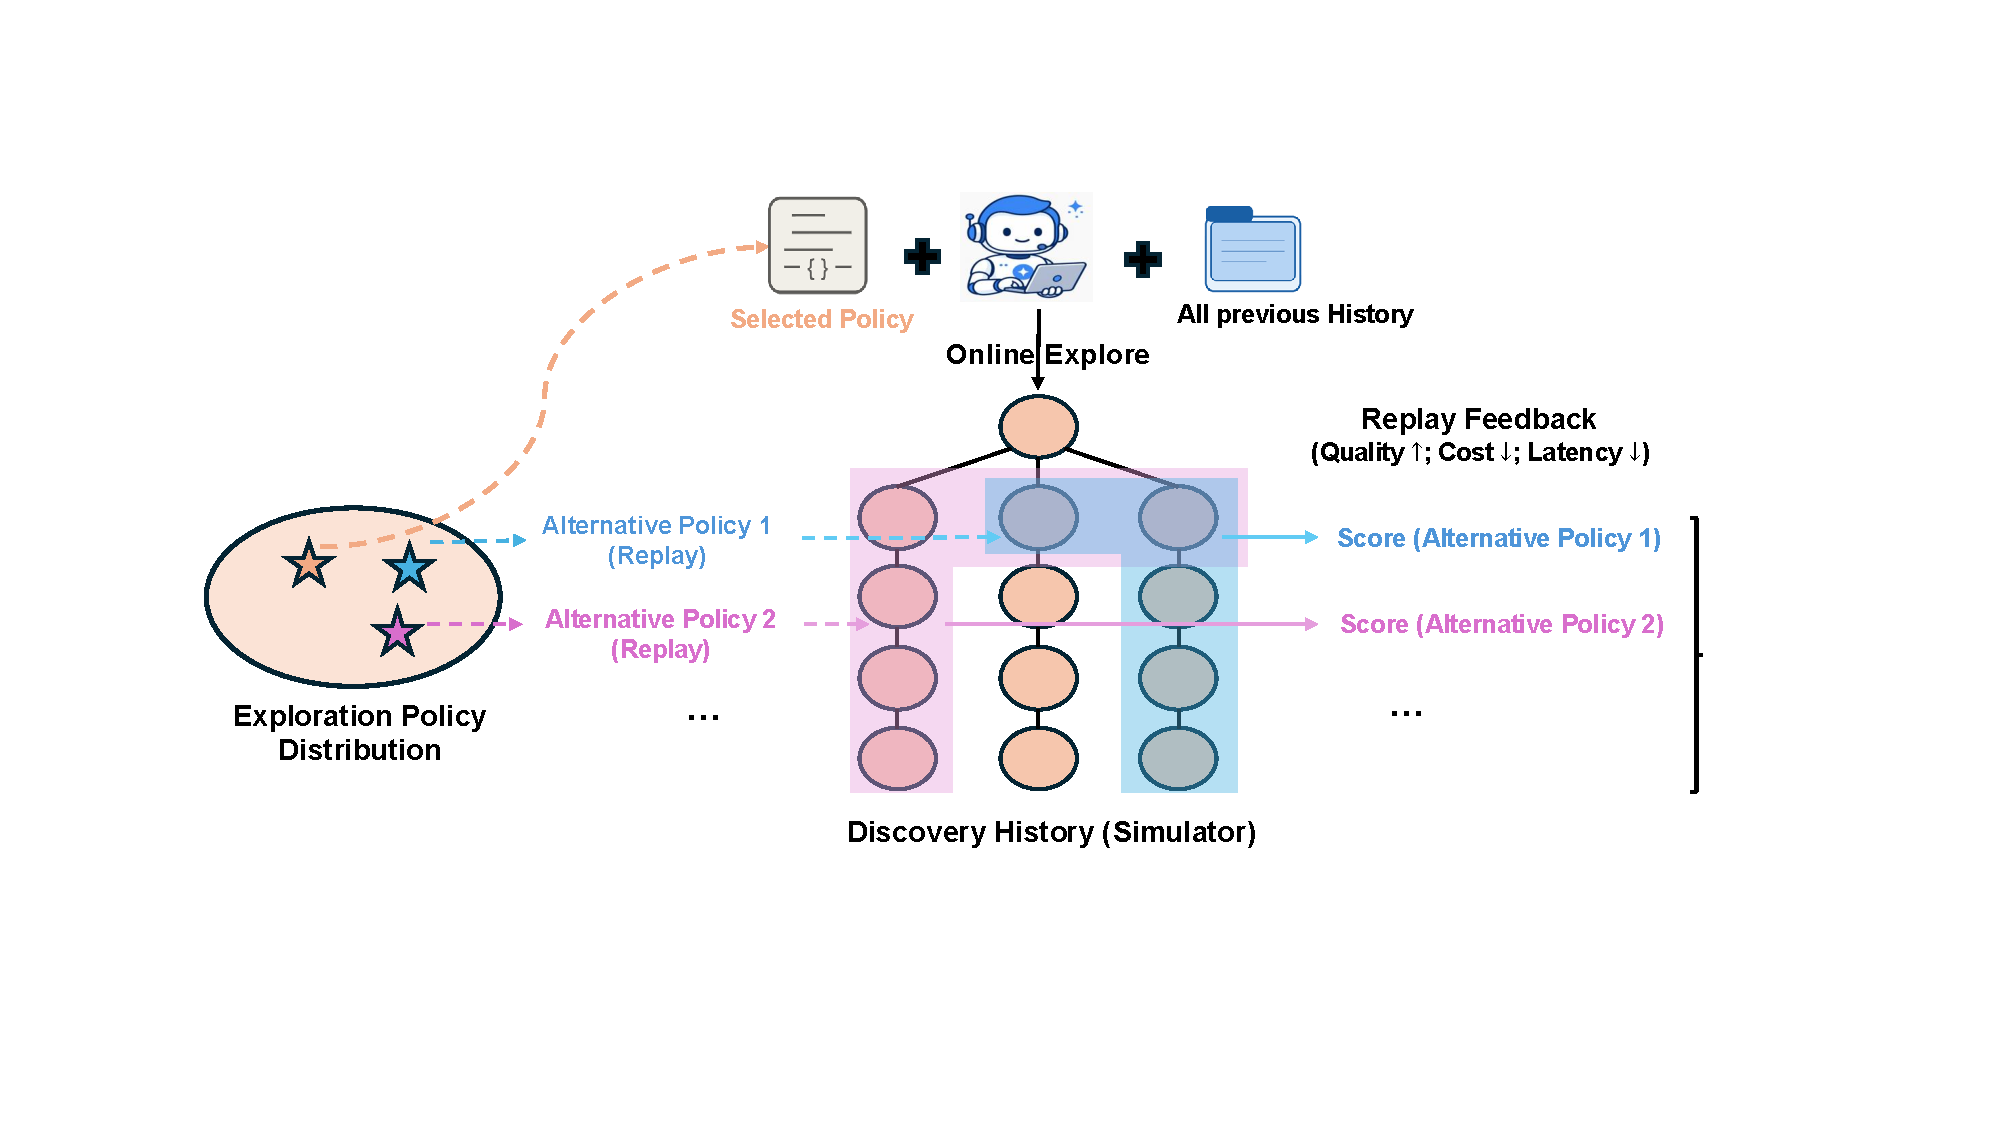
\includegraphics[width=0.92\linewidth]{Main_Text/Figures/HRS-latest.pdf}
    \caption{\textbf{Discovery history as a replay simulator.} A deployed policy first explores online to generate a structured discovery tree containing historical execution traces (each node denote an attempt with its full observation). Thousands of candidate policies can then be tested within this simulator—evaluating alternative choices of search branches, exploration orders, concurrency levels, and stopping rules. \textbf{Since all node outcomes are pre-stored, a single costly online run enables thousands of rapid, zero-execution-cost off-policy evaluations. This enables policy improvement through historical replay: the agent can “dream” over many alternative exploration strategies before redeploying the improved policy online.}}
    \label{fig:motivation}
\end{figure}

\section{Motivation: Discovery History as a Replay Simulator}
% \section{Motivation: Discovery History as a Replayable Environment}
\label{sec:history_environment}

Consider an agent navigating toward a goal in an unfamiliar environment. During its first traversal, the agent may follow inefficient routes, encounter
dead ends, backtrack, and gradually construct a map of the surrounding space. Once recorded, however, this experience becomes reusable: the resulting map
supports planning without requiring the agent to physically revisit every location. A new navigation policy can instead reason over the accumulated map,
avoid known dead ends, reconsider earlier decisions, and compare alternative
routes before acting~\citep{gupta2017cognitive}.

This idea parallels model-based reinforcement learning \citep{SUTTON1990216, m2023model}. A model captures how an environment evolves in response to an agent's actions, allowing policies to be trained or evaluated through simulated experience rather than
repeated interaction with the real environment~\citep{ha2018world}. The Dreamer family~\citep{hafner2019dream, hafner2020mastering, hafner2023mastering, hafner2025training} demonstrates this principle particularly clearly: an agent learns a compact dynamics model from collected experience and improves its policy by imagining trajectories within that model.

Long-horizon discovery admits an analogous structure. An exploration policy decides which directions to pursue, which candidates to refine, which branches to explore in parallel, and when to terminate. Executing the policy online produces a structured discovery history containing the explored branches, decision points, computational costs, and realized outcomes. As illustrated in
Figure~\ref{fig:motivation}, this history can subsequently be treated as an \emph{empirical replay simulator}: a grounded model of the portion of the discovery space that has already been observed.

Within this replay simulator, alternative exploration policies induce different trajectories through the recorded discovery tree. A policy may select a different subset of branches, prioritize them in a different order, issue different requests in parallel, or stop at an earlier point. Evaluating such a trajectory requires only revealing the outcomes already stored along the
selected branches, rather than rerunning the underlying coding agent and evaluator. Consequently, a single expensive online discovery run can support many inexpensive evaluations of alternative exploration strategies.

